    The rough overall approach presented in the motivating example is summarized in short here. Figure \ref{fig:overall_approach} shows the sequential process described in the motivating example. The process starts with a knowledge graph (like Figure \ref{fig:motivating_example_kg}), which gets transformed into a dataset (like Figure \ref{fig:motivating_dataset}). The dataset is in turn used to train a machine learning model like the decision tree in Figure \ref{motivating_example_decision_tree}. Now, constraints like the one about contacts with non-vaccinated persons can be validated over the knowledge graph and the trained machine learning model. Afterward, the constraint satisfaction results can be used for visualizations, meant to explain predictions of the model, show the validity according to the constraint, and might provide inside into patterns used by the model. Figure \ref{motivating_example_annotated_decision_tree} illustrates this visualization.
    
    
    \begin{figure}
        \centering
        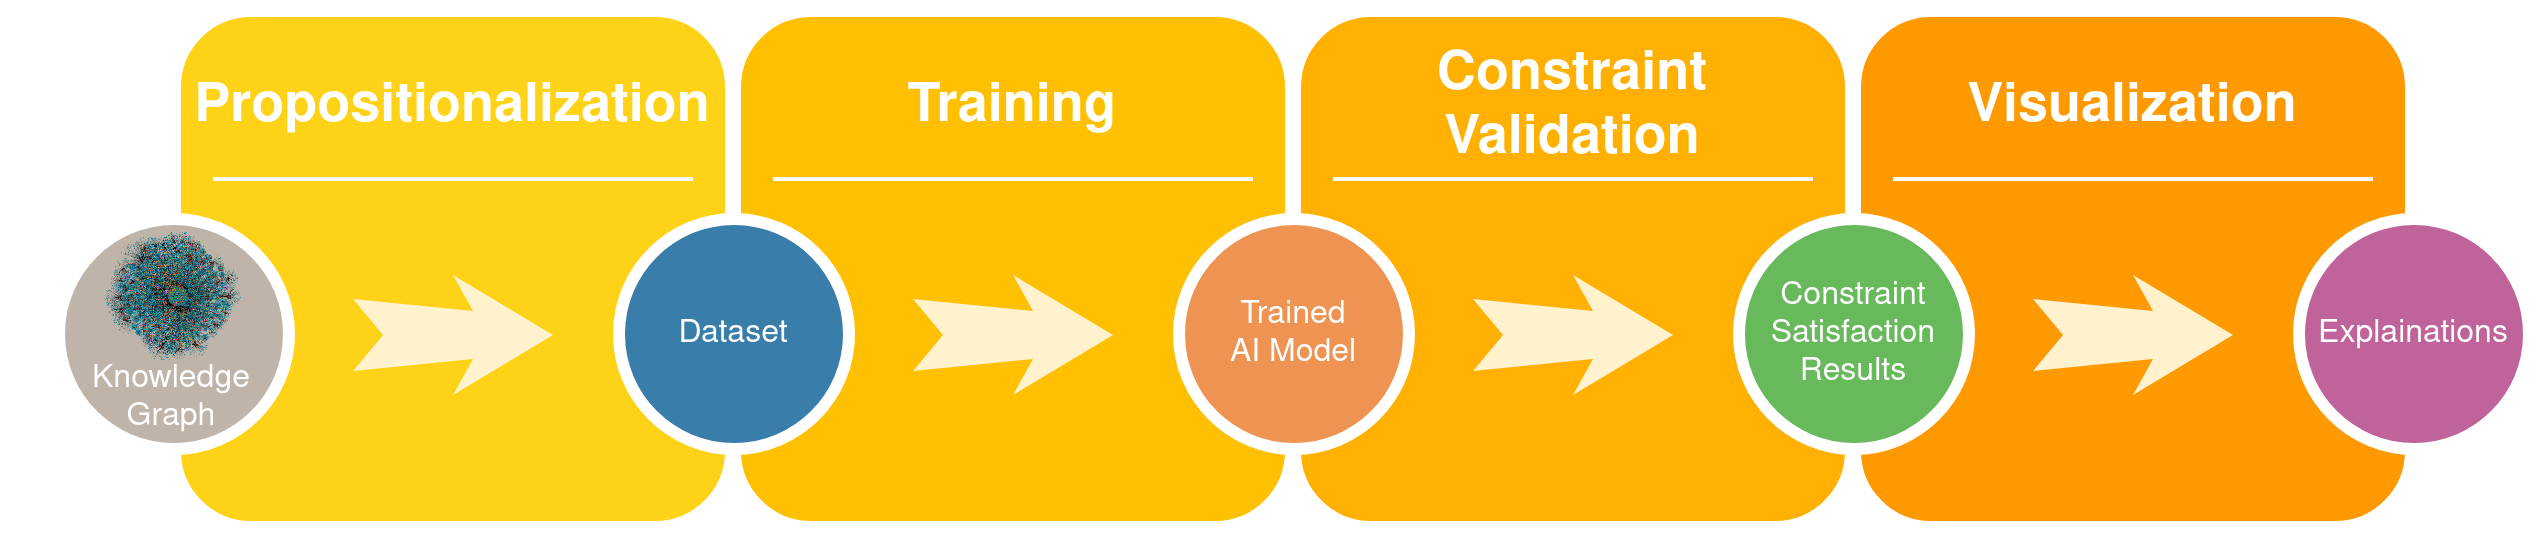
\includegraphics[width=\textwidth]{images/motivating_example/overall_approach.png}
        \caption{Showing the overall approach as a sequential process}
        \label{fig:overall_approach}
    \end{figure}